\documentclass[conference]{IEEEtran}
\IEEEoverridecommandlockouts
% The preceding line is only needed to identify funding in the first footnote. If that is unneeded, please comment it out.
%----------------------------------------------------------
\usepackage{cite}
\usepackage[pdftex]{graphicx}
% declare the path(s) where your graphic files are
\graphicspath{images/}
\DeclareGraphicsExtensions{.pdf,.jpeg,.png,.jpg}
\usepackage{amsmath,amssymb,amsfonts}
\usepackage{algorithmic}
\usepackage{graphicx}
\usepackage{textcomp}
\usepackage{array}
%\usepackage[caption=false,font=normalsize,labelfont=sf,textfon =sf]{subfig}
\usepackage{dblfloatfix}
\usepackage{url}
\usepackage{lipsum}
\usepackage{listings}
\usepackage{xcolor}
\def\BibTeX{{\rm B\kern-.05em{\sc i\kern-.025em b}\kern-.08em
    T\kern-.1667em\lower.7ex\hbox{E}\kern-.125emX}}

\definecolor{mygreen}{rgb}{0,0.6,0}

\lstset{
  breaklines=true,
  frame=single,
  keepspaces=true,
  commentstyle=\color{mygreen},
  keywordstyle=\color{blue},
  showspaces=false,
  showstringspaces=false,
  showtabs=false,
}

%----------------------------------------------------------
    \lstset{
        escapeinside={/*@}{@*/},
        language=Python,	
        basicstyle=\fontsize{8.5}{12}\selectfont,
        numbers=left,
        numbersep=2pt,    
        xleftmargin=2pt,
        frame=tb,
        columns=fullflexible,
        showstringspaces=false,
        tabsize=4,
        keepspaces=true,
        showtabs=false,
        showspaces=false,
        morekeywords={inline,public,class,private,protected,struct},
        captionpos=b,
        lineskip=-0.4em,
        aboveskip=10pt,
        extendedchars=true,
        breaklines=true,
        prebreak = \raisebox{0ex}[0ex][0ex]{\ensuremath{\hookleftarrow}},
        keywordstyle=\color[rgb]{0,0,1},
        commentstyle=\color[rgb]{0.133,0.545,0.133},
        stringstyle=\color[rgb]{0.627,0.126,0.941},
    }
%----------------------------------------------------------

\begin{document}

\title{Controle de braços robóticos auxiliados por visão computacional.
% \\
% {\footnotesize \textsuperscript{*} Sistemas Embarcados: Prof. Marco Reis - marco.reis@ba.docente.senai.brr}
% \thanks{Identify applicable funding agency here. If none, delete this.}
}

% \author{\IEEEauthorblockN{Marco Reis, 41650-010\IEEEauthorrefmark{1}}
% \IEEEauthorblockA{\IEEEauthorrefmark{1}Robotics & Autonomous Systems Center,
% Senai Cimatec, Salvador, Brazil}% <-this % stops an unwanted space


\author{\IEEEauthorblockN{Marco Reis (orientador)}
\IEEEauthorblockA{\textit{SENAI CIMATEC} \\
% \textit{name of organization (of Aff.)}\\
Salvador, Brasil \\
marco.reis@aln.senaicimatec.edu.br}
\and
\IEEEauthorblockN{Tiago Barretto Sant’Anna}
\IEEEauthorblockA{\textit{SENAI CIMATEC} \\
% \textit{name of organization (of Aff.)}\\
Salvador, Brasil\\
tiago.sant'anna@ba.estudante.senai.br}
}

\maketitle

\begin{abstract}
O objetivo deste artigo é expor o desafio de comunicação entre dois Arduinos. Portanto para cumprir com o desafio é necessário receber os dados de distancia através de um sensor ultrassônico de acordo com distancia acende determinado LED e envia o sinal para outro Arduino que exibe em um display LCD. Esse desafio tem como objetivo o aprendizado sobre programação, uso de sensores e comunicação entre dispositivos. Por fim foi possível realizar essa tarefa e adquirir os conhecimentos necessários.

\end{abstract}

\begin{IEEEkeywords}
Arduino, comunicação, sensores, simulação.
\end{IEEEkeywords}

\section{Introdução}

Arduino é uma placa de prototipagem com um microprocessador que permite a realização de projetos de eletrônica com alta facilidade \cite{Arduino:online}. Dessa forma, busca-se realizar uma atividade para aumentar o conhecimento nessas tecnologias. Assim foi realizado uma atividade que consiste em utilizar dois Arduino para se comunicar, um deles sendo responsável por enviar os dados de um sensor ultrassônico e o outro para receber e mostrar em um display lcd os valores de distancia. Com isso busca-se adquirir conhecimentos de programação, uso de sensores e comunicação.

\section{Desenvolvimento}

\subsection{Materiais utilizados}
\begin{itemize}
    \item 2 Arduinos UNO;
    \item 2 protoboards;
    \item display 16x2;
    \item jumpers;
    \item potenciômetro;
    \item resistores;
    \item LEDs de cor vermelha amarela e branca.
\end{itemize}


\subsection{Métodos}

Para a realização do desafio foi necessário realizar um estudo acerca do uso do display no Arduino\cite{display:online}. Logo em seguida foi necessário fazer um estudo sobre como se comunicar com as portas seriais para comunicar com 2 arduinos\cite{Serial:online}. Por fim, foi feito um estudo do funcionamento do sensor ultrassônico e como obter seus dados\cite{Serial:online}.

\subsection{Funcionamento do circuito}

\begin{figure}[h!]
\centering
    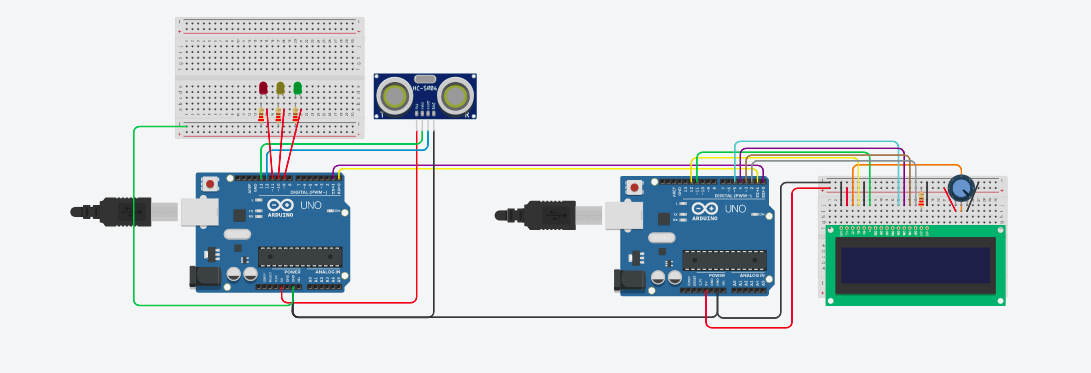
\includegraphics[width=8cm]{images/circuito.jpg}
\caption{Exemplos de tags \cite{OpenCVDe76:online}}
\label{fig:circuito}
\end{figure}

Como mostrado na figura\ref{fig:circuito} o primeiro Arduino é conectado no sensor ultrassônico e nos LEDs. A função deste Arduino é de receber os dados do sensor, acender os LEDs de acordo com a distancia e enviar os dados da distancia para o segundo Arduino.

Desse modo, o segundo Arduino, esta conectado no primeiro e também no display. Sua função é de receber os dados do primeiro e mostra-los no display. O potenciômetro conectado no display tem uma função de controlar o contraste de fundo do display.

\subsection{Código do primeiro Arduino}

\begin{lstlisting}[language=C]
#include <stdio.h>
#include <stdlib.h>
#include <string.h>

// distance sensor
int trigger =13, echo = 12;
int cm = 0;
char num[10];

//leds
int red = 11, yllw = 10, grn = 9; 
\end{lstlisting}

Essa primeira parte do código declara as bibliotecas e variáveis utilizadas no código.

\begin{lstlisting}[language=C]
long readUltrasonicDistance(int triggerPin, int echoPin)
{
  pinMode(triggerPin, OUTPUT);  // Clear the trigger
  digitalWrite(triggerPin, LOW);
  delayMicroseconds(2);
  // Sets the trigger pin to HIGH state for 10 microseconds
  digitalWrite(triggerPin, HIGH);
  delayMicroseconds(10);
  digitalWrite(triggerPin, LOW);
  pinMode(echoPin, INPUT);
  // Reads the echo pin, and returns the sound wave travel time in microseconds
  return pulseIn(echoPin, HIGH);
}
\end{lstlisting}

Essa função foi inspirada nos estudos feitos\cite{sensor:online} e corresponde ao sensor ultrassônico. Ela funciona calculando o tempo da viagem da onda do sensor e multiplicando por uma constante.

\begin{lstlisting}[language=C]
void setup()
{
  Serial.begin(9600);
  pinMode(red, OUTPUT);
  pinMode(yllw, OUTPUT);
  pinMode(grn, OUTPUT);
}
\end{lstlisting}

Esse código define o \textit{baud rate}, que é a taxa de transmissão de dados e os pinos de saída dos LEDs.

\begin{lstlisting}[language=C]
void loop()
{
  // measure the ping time in cm
  cm = 0.0175 * readUltrasonicDistance(trigger, echo);
  itoa(cm,num,10);
\end{lstlisting}

Essa parte do código recebe o dado da distancia em valor \textit{long} e transforma em dado do tipo \textit{String} para que possa ser enviado pela porta serial.

\begin{lstlisting}[language=C]
  if(cm < 100){
    Serial.write("Regiao1:");
    Serial.write(num);
    Serial.write(" ");
    digitalWrite(red, HIGH);
    
  } else if(100 <= cm && cm < 200){
    Serial.write("Regiao2:");
    Serial.write(num);
    digitalWrite(yllw, HIGH);
    
  } else{
    Serial.write("Regiao3:");
    Serial.write(num);
    digitalWrite(grn, HIGH);
  }
  Serial.write('\n');
  delay(300);
  digitalWrite(red, LOW);
  digitalWrite(yllw, LOW);
  digitalWrite(grn, LOW);
}
\end{lstlisting}

Essa parte é responsável por acender os LEDs e enviar os dados pela porta serial.

\subsection{Código do segundo arduino}

\begin{lstlisting}[language=C]
#include <LiquidCrystal.h>
// Reciever
char mystr[20]; //Initialized variable to store recieved data
char resp[20];
// Define os pinos que serao utilizados para ligacao ao display
LiquidCrystal lcd(12, 11, 5, 4, 3, 2);
\end{lstlisting}

Essa parte define a variável que recebe a resposta e os pinos do display.


\begin{lstlisting}[language=C]
void setup()
{
  // Define o numero de colunas e linhas do LCD
  lcd.begin(16, 2);
  Serial.begin(9600);
}
\end{lstlisting}

Nessa parte é definido o \textit{baud rate} e inicializa o display.

\begin{lstlisting}[language=C]
    void loop()
{
  if(Serial.available() > 0){
    Serial.readBytes(mystr,11);
    lcd.setCursor(0, 0);
    if(mystr[0] == 'R'){
      lcd.print(mystr);
      delay(100);
      Serial.write(resp);
      break;
    }
  }
 
 delay(300);
 
 lcd.clear();
}
\end{lstlisting}

Esta parte consiste em verificar se a porta serial esta disponivel e logo depois verificar se o sinal esta sendo enviado da maneira correta.

\section{Conclusão}

Com a finalização do desafio foi possível compreender e obter conhecimentos acerca da programação em Arduino, uso do sensor ultrassônico e da comunicação serial.

%----------------------------------------------------------
\bibliographystyle{IEEEtran}
\bibliography{Bibliography}
%CRITICAL: do not change the above two lines!!!
%----------------------------------------------------------

% \vspace{12pt}
% \color{red}
% Course templates contain guidance text for composing and formatting Course papers. Please ensure that all template text is removed from your course paper prior to submission to the lecturer. Failure to remove the template text from your paper may result in your paper not being accepted.

\end{document}
